\chapter{Síntesis de software para GNC embebido}
\label{ch:especifico2}

Como se pudo observar en el capítulo \ref{ch:especifico1}, se realizó la selección de la tarjeta de desarrollo Zedboard para el desarrollo del proyecto, además de esto uno de los parámetros que se tomó en cuenta fue la compatibilidad de esta con el flujo de trabajo de Yocto Project.

\begin{figure}[h!]
    \centering
    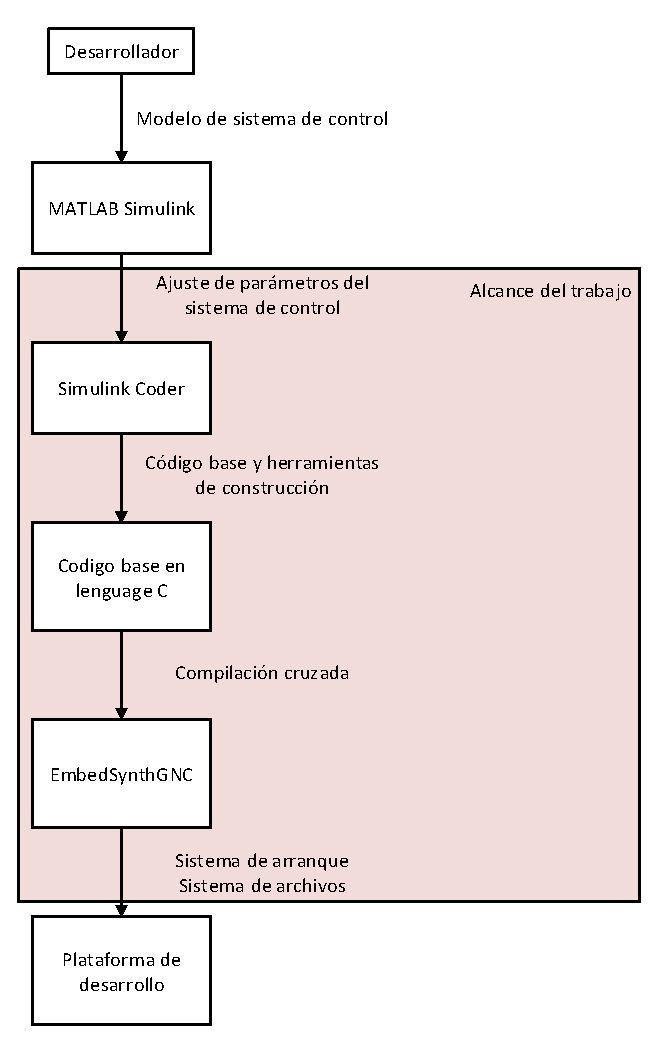
\includegraphics[width=0.48\textwidth]{fig/especifico_2/Diagrama general del proyecto.pdf}
    \caption{Diagrama general del flujo de trabajo propuesto}
    \label{fig:diagrama_flujo_trabajo}
\end{figure}

En este capítulo se pretenden establecer los flujos de trabajo para el prototipado de algoritmos de control de orientación y navegación para aplicaciones espaciales. Esto mediante la implementación de un caso de estudio. Como se puede observar en la Figura \ref{fig:diagrama_flujo_trabajo}, primeramente el desarrollador toma un modelo de sistema de control el cual implementa en MATLAB Simulink por medio de los bloques del sistema. 

Seguido de esto se realiza un ajuste de parámetros con el objetivo que el mismo opere dentro de las condiciones esperadas, una vez ajustado el sistema se debe de ingresar el modelo al flujo de trabajo de Simulink Coder, el cual nos dará como salida el código base y las herramientas de construcción requeridas para poder compilar el archivo ejecutable, cabe destacar que la compilación a realizar es cruzada, esta nos permite compilar los archivos en un sistema distinto al objetivo. 

Finalmente se debe de ingresar el archivo binario generado al flujo de trabajo de EmbedSynthGNC, el cual, se encargara de dar como salida un archivo de arranque y el sistema de archivos listos para implementar en la plataforma de desarrollo.


\section{Creación de los entornos de desarrollo}

En esta sección se describen los pasos necesarios para la creación de los entornos de desarrollo utilizados en este proyecto. En el mismo se incluye la información del hardware y software utilizado, además de las versiones de los sistemas requeridos para cada una de las implementaciones. 

\subsection{MATLAB}\label{subsec:generacion_entorno_matlab}
Primeramente se describirá el hardware utilizado para ejecutar MATLAB y sus herramientas, la versión utilizada es MATLAB 2024b por medio de una licencia de prueba de la versión full, esta misma se ejecuta en una computadora con las siguientes características: 
\begin{itemize}
    \item Procesador Intel i9 - 14900k 
    \item Almacenamiento 500 GB 
    \item Memoria 16 GB
    \item Video Nvidia RTX4060Ti
\end{itemize}

Las herramientas adicionales instaladas en el entorno de MATLAB son:

\begin{itemize}
    \item Simulink
    \item MATLAB Coder
\end{itemize}

Además de esto se instala la herramienta GCC en su versión 6.3.0, el cual es el compilador de código C, este se utilizara para compilar el código y probar que el mismo funcione de la forma esperada; cabe destacar, que este no es el compilador cruzado, este compilador nos genera un archivo binario el cual podremos probar en el sistema Windows, esto con el fin de poder realizar correcciones más eficientes al sistema de control en caso de ser requerido.

\subsection{Contenedores}

En la elaboración del proyecto se decanta por el uso de contenedores, ya que como se mencionó en \ref{sec:containers}, estos permiten encapsular todas las dependencias y configuraciones necesarias para ejecutar una aplicación. Esto asegura que la misma aplicación funcione de manera consistente en diferentes entornos, ya sea durante el desarrollo, en pruebas o en producción. 

Cada contenedor opera de forma independiente, lo que permite ejecutar múltiples aplicaciones en el mismo sistema sin interferencias. Este aislamiento reduce significativamente el riesgo de conflictos entre diferentes versiones de software y dependencias, lo que se traduce en un entorno más estable y predecible. Los contenedores se ejecutan en un sistema operativo Linux en su versión 22.04 LTS.

El sistema donde se ejecutan los contenedores cuenta con las siguientes características:

\begin{itemize}
    \item Procesador Intel i9 - 14900k
    \item Almacenamiento 500 GB 
    \item Memoria 16 GB
    \item Video Nvidia RTX4060Ti
\end{itemize}

Una vez que se hayan comprendido el sistema operativo y las características del hardware del computador anfitrión, se presentarán los comandos básicos para la creación y gestión de contenedores.

\subsubsection{Comandos utilizados para la creación y gestión de contenedores}\label{subsec:manejo_de_contenedores}


\begin{lstlisting}[language=bash, caption={Instalacion de docker, Linux}, label=lst:install_docker]
    sudo apt install docker.io
\end{lstlisting}

Como se puede observar mediante el uso de \ref{lst:install_docker}, se realiza la instalación de docker.io, el cual como se mencionó en \ref{sec:containers}, es una plataforma que permite la creación, despliegue y gestión de aplicaciones en contenedores. 

\begin{lstlisting}[language=bash, caption={Instalacion de Ubuntu 20.04, Linux}, label=lst:install_20_04_ubuntu]
    sudo docker run -it ubuntu:20.04 /bin/bash
\end{lstlisting}

Por medio del comando \ref{lst:install_20_04_ubuntu} se realiza la construccion de la máquina dentro del entorno del contenedor. Este último comando se encarga de descargar la imagen de Ubuntu 20.04, crea y ejecuta un contenedor en modo interactivo además de proporcionar acceso al terminal del contenedor, donde se ejecutan comandos como si fuera una máquina virtual con Ubuntu 20.04. Este contenedor será utilizado para realizar la compilación cruzada, se utiliza Ubuntu 20.04, ya que esta versión contiene la versión de GCC que satisface los requerimientos impuestos por otros flujos de trabajo.

\begin{lstlisting}[language=bash, caption={Instalacion de Ubuntu 16.04, Linux}, label=lst:install_16_04_ubuntu]
    sudo docker run -it ubuntu:16.04 /bin/bash
\end{lstlisting}

Por otro lado por medio del comando mostrado en \ref{lst:install_16_04_ubuntu}, se genera el contenedor que se utilizara para la implementación del flujo de trabajo de Yocto Project, cabe destacar que se utiliza Ubuntu 16.04, ya que, es la versión que cumple con los requerimientos del flujo de trabajo de Yocto, esto se debe a que al trabajar con Yocto Zeus y este ser desarrollado en el año 2019, esta era la versión de Ubuntu más estable para la fecha. 

\begin{lstlisting}[language=bash, caption={Lista de contenedores del sistema, Docker}, label=lst:docker_basics_ps-a]
    sudo docker ps -a
\end{lstlisting}

\begin{figure}[h!]
    \centering
    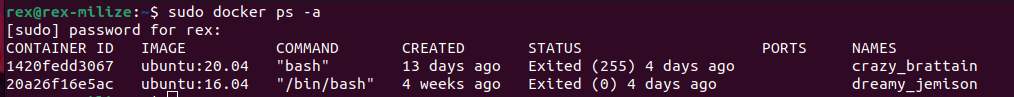
\includegraphics[width=0.85\textwidth]{fig/especifico_2/retornos_de_comandos/sudo_docker_ps_a.png}
    \caption{Retorno del comando \ref{lst:docker_basics_ps-a}}
    \label{fig:sudo_docker_ps_a}
\end{figure}

Una vez generados los dos contenedores, los mismos podrán ser consultados mediante el comando que se muestra en \ref{lst:docker_basics_ps-a}, este se encarga de devolver una lista como la que se muestra en \ref{fig:sudo_docker_ps_a}, donde se puede observar de izquierda a derecha las columnas denominadas: Container ID, el cual es el identificador del contenedor, este valor se debe de utilizar para referirse al contenedor para las operaciones que se realizan fuera del entorno, también se muestra la Imagen que el contenedor tiene instalada, el comando de creación del mismo, la creación del contenedor, el status, los puertos definidos y el Nombre.

Para efectos de este proyecto se tomará importancia solamente a las columnas de Container ID e Imagen.

\begin{lstlisting}[language=bash, caption={Iniciar un contenedor, Docker}, label=lst:docker_basics_start]
    sudo docker start <ID del contenedor>
\end{lstlisting}

\begin{figure}[h!]
    \centering
    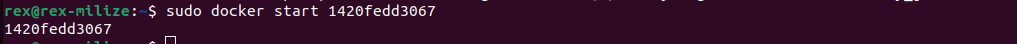
\includegraphics[width=0.85\textwidth]{fig/especifico_2/retornos_de_comandos/sudo_docker_start.png}
    \caption{Retorno del comando \ref{lst:docker_basics_start}}
    \label{fig:sudo_docker_start}
\end{figure}

Por medio del comando que se muestra en \ref{lst:docker_basics_start} se inicia el contenedor deseado, esto siempre dependerá del ID que se coloque, tras la ejecución de este comando la salida del mismo se puede observar en la Figura \ref{fig:sudo_docker_start}

\begin{lstlisting}[language=bash, caption={Ingresar a un contenedor, Docker}, label=lst:docker_basics_init]
    sudo docker exec -it <ID del contenedor> \bin\bash
\end{lstlisting}

\begin{figure}[h!]
    \centering
    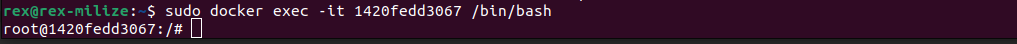
\includegraphics[width=0.85\textwidth]{fig/especifico_2/retornos_de_comandos/sudo_docker_init.png}
    \caption{Retorno del comando \ref{lst:docker_basics_init}}
    \label{fig:sudo_docker_init}
\end{figure}

Finalmente, para la ejecución del contenedor en terminal se debe de hacer uso del comando \ref{lst:docker_basics_init}, este se encarga de acceder a la terminal del contenedor deseado. Como se puede observar en la Figura \ref{fig:sudo_docker_init} ya la terminal se encuentra ejecutando el contenedor construido bajo el ID del contenedor "1420fedd3067".

Una vez generados los contenedores, se procede a generar el entorno de desarrollo requerido dentro de los mismos.

\subsubsection{Contenedor para compilación Cruzada}\label{subsec:generacion_entorno_xcompile}

Este contenedor será en el cual se lleve a cabo la compilación cruzada, es por esto que el mismo contendrá las herramientas que se mencionan a continuación:

\begin{itemize}
    \item Compilador cruzado el cual sea compatible con la plataforma de desarrollo
    \item Constructor de archivos
\end{itemize}

\begin{lstlisting}[language=bash, caption={Instalacion del compilador cruzado, Contenedor}, label=lst:cross_compiler]
    sudo apt install gcc-arm-linux-gnueabihf
\end{lstlisting}

\begin{lstlisting}[language=bash, caption={Instalacion de CMake, Contenedor}, label=lst:cmake]
    sudo apt install cmake
\end{lstlisting}

\begin{lstlisting}[language=bash, caption={Instalacion de build essential, Contenedor }, label=lst:build_essential]
    sudo apt install build-essential
\end{lstlisting}

Una vez generado el contenedor debemos de instalar en el mismo el compilador cruzado que para nuestros efectos será arm-linux-gnueabihf-gcc, esto lo podemos hacer mediante el comando que se muestra en \ref{lst:cross_compiler},  CMake el cual es una herramienta de construcción multiplataforma y de código abierto que se utiliza para gestionar la construcción de software utilizando un enfoque basado en proyectos y finalmente build-essential las cuales son herramientas que nos ayudaran a compilar el programa generado.


\subsubsection{Contenedor para Yocto Project}\label{subsec:generacion_entorno_yocto}

El contenedor para Yocto Project, será en el cual se lleve a cabo la construcción de la imagen a utilizar en la plataforma de desarrollo, para esto se requiere la instalación de algunas dependencias las cuales se mencionan a continuación:

\begin{itemize}
    \item Instalacion de tree 
    \item Instalacion de vim
    \item Creación de un usuario no Root
    \item Yocto Project
\end{itemize}

\subsubsection{Creación de un usuario no root}

Para el uso del marco de trabajo de Yocto se debe de generar un usuario no root, esto principalmente por razones de seguridad y manejo adecuado de permisos. El usuario se puede generar por medio de los siguientes comandos:

\begin{lstlisting}[language=bash, caption={Generacion de usuario no root, Linux}, label=lst:no_root_user]
    apt - get install -y sudo
    useradd - ms/bin/bash myuser
    echo "myuser:password" | chpasswd
    usermod - aG sudo myuser
\end{lstlisting}

De forma que según el comando observado en \ref{lst:no_root_user}, en la primera línea instalamos sudo, seguido de esto en la segunda línea se agrega el usuario denominado "myuser", en la tercera línea se genera una contraseña para este usuario la cual se define como "chpasswd", finalmente se agrega en el archivo usermod el nuevo usuario. 

\begin{lstlisting}[language=bash, caption={Iniciar usuario no root, Linux}, label=lst:no_root_user_log]
    su - myuser
\end{lstlisting}


Cada vez que iniciemos el contenedor siempre lo haremos como usuario root, para poder iniciar con el usuario no root llamado "myuser" se debe de hacer uso del comando que se muestra en \ref{lst:no_root_user_log}.

\subsubsection{Yocto Project}

Como se observó en \ref{subsec:yocto}, yocto presenta flexibilidades a la hora de configurar un sistema permitiendo al desarrollador seleccionar paquetes específicos y personalizar el sistema operativo.

\begin{lstlisting}[language=bash, caption={Requerimientos Yocto Zeus, Linux}, label=lst:yocto_requirements]
    sudo apt - get install gawk wget git - core diffstat unzip texinfo
    gcc - multilib build - essential chrpath socat cpio python python3
    python3 - pip python3 - pexpect xz - utils debianutils 
    iputils - ping python3 - git python3 - jinja2 
    libegl1 - mesa libsdl1 .2 - dev pylint3 xterm
\end{lstlisting}

Para que el mismo funcione de forma correcta debemos de instalar los requerimientos del marco de trabajo los cuales se pueden observar en \ref{lst:yocto_requirements}.

\begin{lstlisting}[language=bash, caption={Version de Yocto}, label=lst:yocto_clone]
    git clone -b zeus https://git.yoctoproject.org/git/poky
    cd poky
\end{lstlisting}

\begin{lstlisting}[language=bash, caption={BSP para Zedboard}, label=lst:yocto_zedboard]
    git clone -b zeus https://github.com/Xilinx/meta-xilinx
    git clone -b zeus https://github.com/openembedded/meta-openembedded.git
\end{lstlisting}

La versión de yocto a utilizar se debe de clonar de \ref{lst:yocto_clone}, seguido de esto se debe de ir a la rama de la versión Yocto Zeus. Además de clonar este repositorio se debe de ingresar al directorio denominado poky y clonar dentro del repositorio \ref{lst:yocto_zedboard} el cual contiene en su rama llamada Zeus la versión de paquete de soporte para la tarjeta requerida para generar una imagen para la tarjeta de desarrollo seleccionada.

\begin{lstlisting}[language=bash, caption={Configuraciones adicionales, Yocto}, label=lst:aditional_config]
    source oe - init - build - env
    
    echo "MACHINE ??=\"zedboard-zynq7\"" >> conf/local.conf
    echo "IMAGE_FEATURES +=\"package-management\"" >> conf/local.conf
    echo "DISTRO_HOSTNAME =\"zynq\"" >> conf/local.conf
    
    bitbake-layers add-layer ../meta-xilinx/meta-xilinx-bsp/
    bitbake-layers add-layer ../meta-openembedded/meta-oe/
\end{lstlisting}

Algunas configuraciones adicionales que se deben de realizar se muestran en \ref{lst:aditional_config}.


\section{Selección del caso de estudio}

Como caso de estudio se seleccionó una aplicación la cual permitiera una comparación de resultados antes del procesado y después del mismo, es por esto que se decidió implementar un filtro  de tipo paso bajo haciendo uso de los siguientes bloques de MATLAB Simulink. 

\begin{itemize}
    \item Onda seno
    \item Suma
    \item Función de transferencia
    \item Generador de archivo de salida
\end{itemize}

La configuración seleccionada para el primer generador de onda seno es:

\begin{itemize}
    \item Amplitud = 1
    \item Bias = 0 
    \item Frecuencia = 1 rad/s
    \item Fase = 0 
    \item Tiempo de muestreo = 0 
\end{itemize}

Por otro lado, para la segunda onda se tiene la configuración:

\begin{itemize}
    \item Amplitud = 1
    \item Bias = 0 
    \item Frecuencia = 12 rad/s
    \item Fase = 0 
    \item Tiempo de muestreo = 0 
\end{itemize}

Ya que al sumar ondas de diferentes frecuencias, se puede observar un fenómeno llamado modulación, donde la onda resultante presenta un patrón que varía en el tiempo.

\begin{equation}
    y(t) = \sin(t) + \sin(12t)
    \label{eq:funcion_de_suma_de_ondas}
\end{equation}

Por otro lado la función de transferencia a utilizar en el filtro será:

\begin{equation}
    H(S) = \frac{1}{S+1}
    \label{eq:funcion_de_transferencia_filtro}
\end{equation}

Al aplicar el filtro a la señal compuesta,  la onda $\sin(t)$ pasará a través del filtro con poca atenuación, mientras que la onda $\sin(12t)$ será significativamente atenuada debido a su  alta frecuencia.

\begin{figure}[h!]
    \centering
    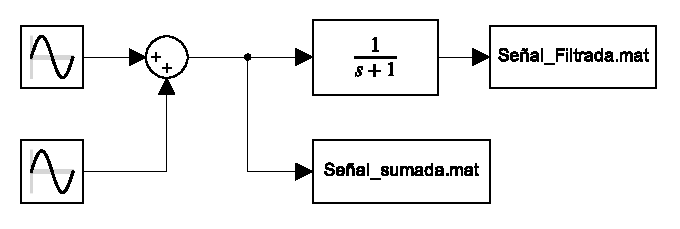
\includegraphics[width=0.5\textwidth]{fig/especifico_2/Diagrama matlab simulink.pdf}
    \caption{Diagrama MATLAB Simulink}
    \label{fig:diagrama_matlab_simulink}
\end{figure}

Estos bloques mencionados anteriormente se colocan como se muestra en la Figura \ref{fig:diagrama_matlab_simulink} de modo que se obtienen como salida del sistema dos archivos, uno llamado señal sumada el cual contiene los datos crudos de la suma de las dos señales y otro denominado señal filtrada el cual contiene los datos de la señal filtrada por la función de transferencia.

\subsection{Simulación del caso de estudio en MATLAB Simulink}\label{subsec:simulacion_caso_de_estudio}

\begin{figure}[h!]
    \centering
    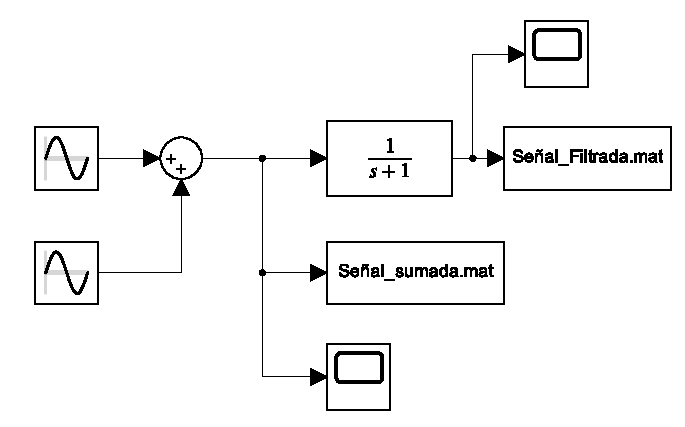
\includegraphics[width=0.5\textwidth]{fig/especifico_2/Diagrama matlab simulink scope.pdf}
    \caption{Diagrama MATLAB Simulink para poder observar las salidas}
    \label{fig:diagrama_matlab_simulink_graficos}
\end{figure}

Utilizando el diagrama de la Figura \ref{fig:diagrama_matlab_simulink}, además de los parámetros configurados anteriormente se colocan dos bloques de gráfico en el diagrama como se muestra en la Figura \ref{fig:diagrama_matlab_simulink_graficos}, esto con el objetivo de poder observar las señales de salida en cada uno de los puntos de interés. 


\begin{figure}[htbp]
    \centering
    \begin{subfigure}[b]{0.45\textwidth}
        \centering
        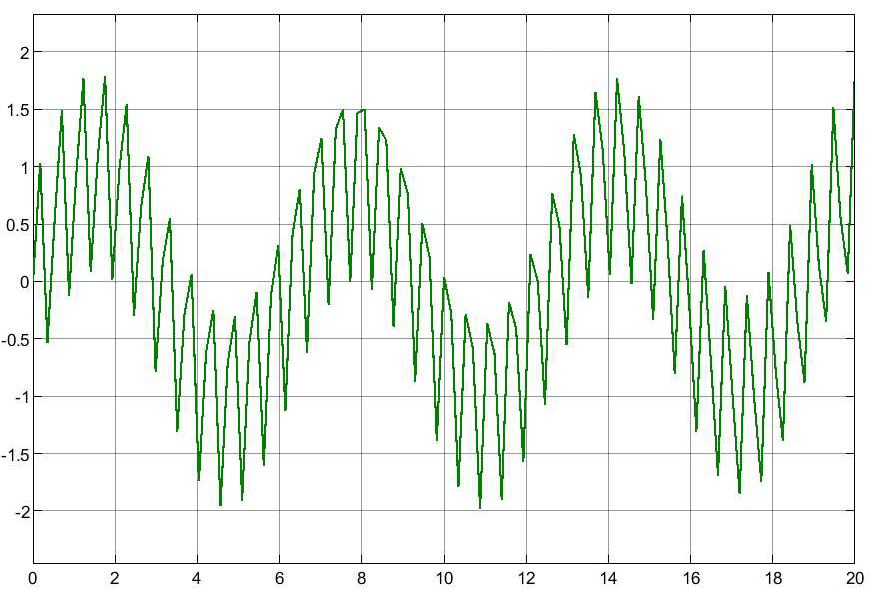
\includegraphics[width=\textwidth]{fig/especifico_2/onda_modulada.pdf}
        \caption{Ondas Moduladas}
        \label{fig:onda_modulada}
    \end{subfigure}
    \hfill
    \begin{subfigure}[b]{0.45\textwidth}
        \centering
        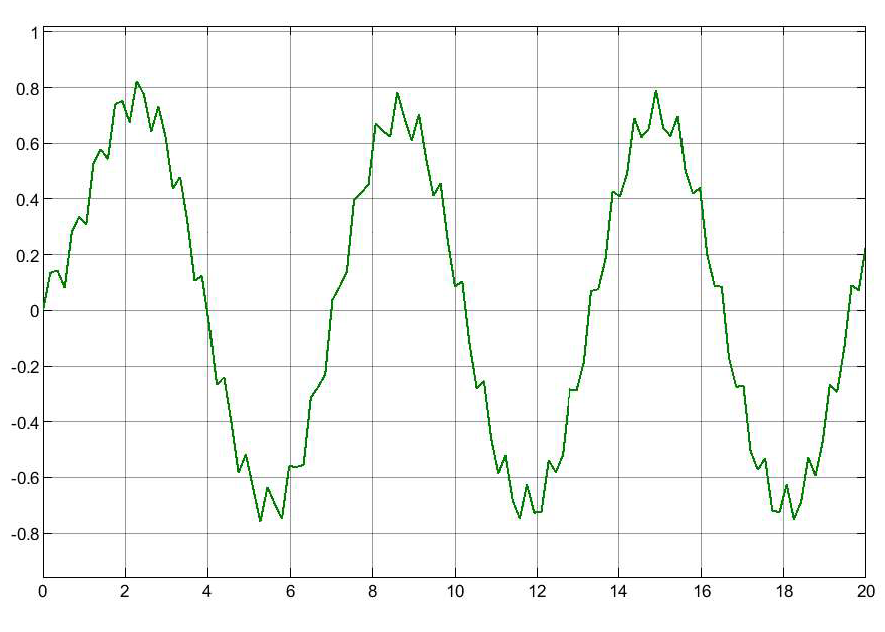
\includegraphics[width=\textwidth]{fig/especifico_2/onda_filtrada.pdf}
        \caption{Onda resultante luego de la función de transferencia}
        \label{fig:onda_filtrada}
    \end{subfigure}
    \caption{Salida simulada del diagrama mostrado en la Figura \ref{fig:diagrama_matlab_simulink_graficos}}
    \label{fig:salida_resultante_diagrama_graficos}
\end{figure}


Como se puede observar en la Figura \ref{fig:onda_modulada} se puede observar la salida de la suma de las dos señales senoidales, por otro lado en la Figura \ref{fig:onda_filtrada} se puede observar la salida de la función de transferencia.

\subsubsection{Resultados obtenidos con la ejecución de la simulación}

Como se mencionó anteriormente los resultados obtenidos se pueden observar en la Figura \ref{fig:salida_resultante_diagrama_graficos}, siendo la salida esperada de la función de transferencia, ya que al ser un filtro paso bajo atenúa las señales que estén por debajo de la frecuencia de corte, que para este filtro es de 1 $rad/s$. Como la señal compuesta contiene una onda seno con frecuencia de 1 $rad/s$ y otra con frecuencia de 12 $rad/s$ es posible observar aun componentes de la frecuencia atenuada.

\section{Flujo de trabajo de la aplicación de transformación de modelo a modelo}

Para poder cumplir con el objetivo de embeber el sistema, se debe de hacer uso del MATLAB Simulink Coder, el cual tiene la capacidad de convertir un sistema de control generado en MATLAB Simulink, en un código C. Algunos de los parámetros que se pueden configurar en este transformador de modelos son: parámetros de la solución, implementación en hardware y generación de código.

A lo largo de este capítulo se definirán los parámetros que se deben de utilizar y el funcionamiento de estos dentro de la generación del código C.

\subsection{Simulink Coder}\label{subsec:simulink_coder}

Una vez comprobado el comportamiento esperado por el caso de estudio se puede proceder con la ejecución del flujo de trabajo de MATLAB Simulink Coder, esto con el fin de transformar el modelo generado en Simulink a un modelo de lenguaje de programación C. Cabe destacar que para esta implementación se utilizó el diagrama que se muestra en la Figura \ref{fig:diagrama_matlab_simulink}, ya que, este solamente contiene como salida los archivos con los datos numéricos del sistema y no contiene las salidas gráficas agregadas en \ref{subsec:simulacion_caso_de_estudio}.


\subsection{Definición de parámetros}

\begin{figure}[h!]
    \centering
    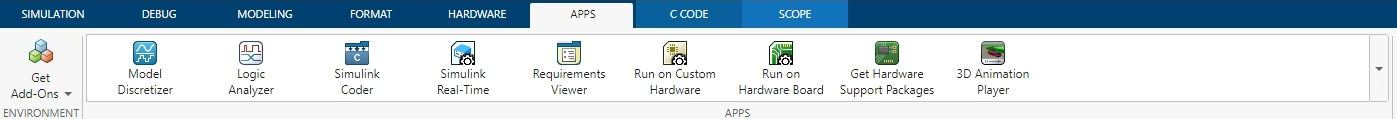
\includegraphics[width=0.8\textwidth]{fig/especifico_2/paso_a_paso_mtmt/apps.png}
    \caption{Pestaña Aplicaciones}
    \label{fig:pestana_apps}
\end{figure}

\begin{figure}[h!]
    \centering
    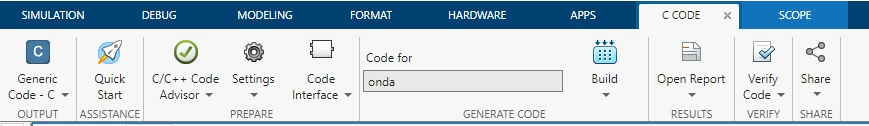
\includegraphics[width=0.8\textwidth]{fig/especifico_2/paso_a_paso_mtmt/c_code.png}
    \caption{Pestaña código C}
    \label{fig:pestana_c_code}
\end{figure}

\begin{figure}[h!]
    \centering
    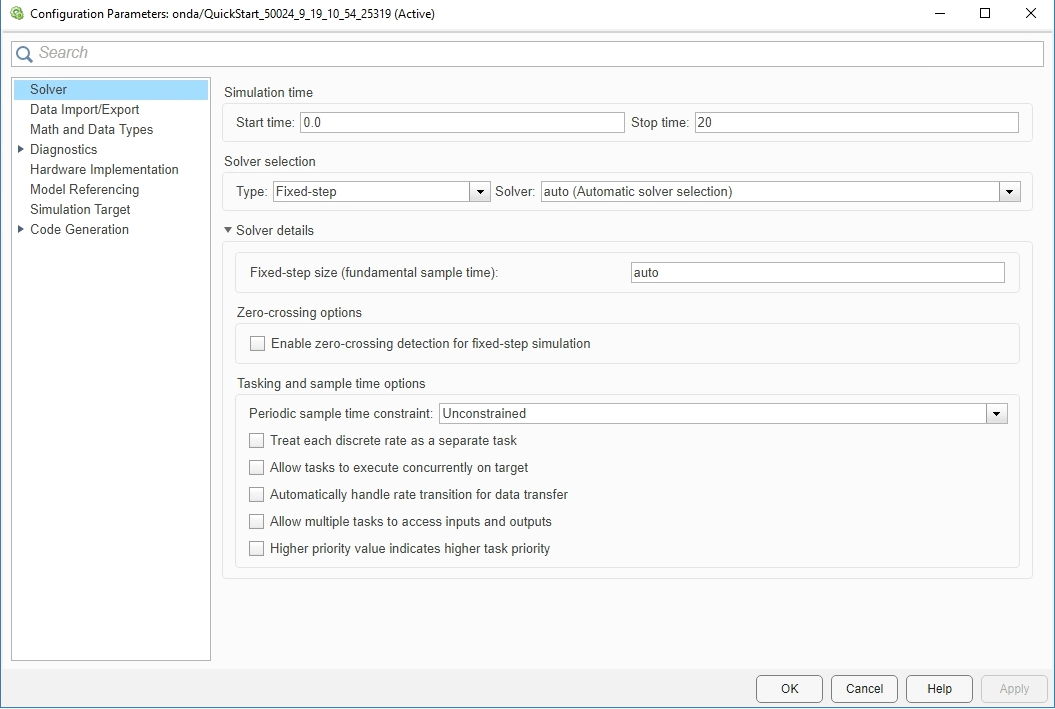
\includegraphics[width=0.8\textwidth]{fig/especifico_2/paso_a_paso_mtmt/configuration_parameters.png}
    \caption{Configuración de parámetros}
    \label{fig:pestana_config}
\end{figure}

Para la definición de parámetros, se debe de estar en el entorno de MATLAB Simulink, una vez en el entorno mencionado anteriormente se debe ir a la pestaña denominada Aplicaciones, o bien APPS como se muestra en la Figura \ref{fig:pestana_apps}, se deberá de seleccionar la aplicación denominada Simulink Coder, cuando seleccionamos esta opción se abrirá una pestaña llamada código C, o bien C CODE como se pudo observar en la Figura \ref{fig:pestana_c_code}.

Una vez estemos en la pestaña de código C, debemos de ir a la opción de configuración de parámetros, en la Figura \ref{fig:pestana_c_code} se observa esta opción bajo el nombre de settings, una vez presionada la opción se abre una ventana emergente como la que se muestra en la Figura \ref{fig:pestana_config}, en la pestaña denominada Solver se deberán de proporcionar los datos sobre el tiempo de ejecución de la prueba.

\subsubsection{Selección del procesador objetivo}

\begin{figure}[h!]
    \centering
    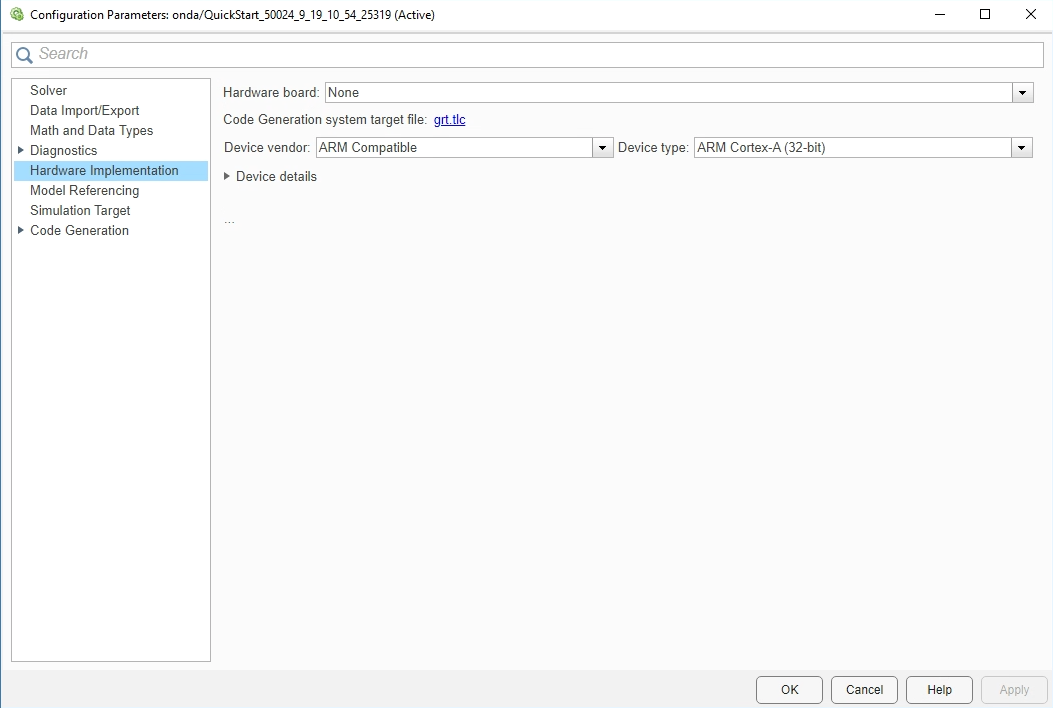
\includegraphics[width=0.8\textwidth]{fig/especifico_2/paso_a_paso_mtmt/configuration_parameters_processor.png}
    \caption{Selección del procesador y la familia del procesador}
    \label{fig:pestana_config_procesador}
\end{figure}

Continuando en la sección de configuración de parámetros ahora debemos de ir a la pestaña llamada implementación de hardware o bien Hardware Implementation, en donde deberemos de colocar los datos de Device Vendor el cual hace referencia al tipo de procesador que contiene la tarjeta de desarrollo, para nuestro caso sería ARM Compatible y el Device Type que seria a la familia que pertenece el procesador, para nuestro caso sería un ARM Cortex-A de 32-bits tal y como se muestra en la Figura \ref{fig:pestana_config_procesador}.


\subsubsection{Selección del tipo de archivo de construcción}

Anteriormente configuramos los parámetros de tiempo de operación y procesador de la tarjeta de desarrollo, ahora debemos de configurar el tipo de archivo que se utilizara para la generación de los archivos binarios, como se deberá de realizar una compilación cruzada se debe de elegir un tipo de archivo el cual nos permita compilar los binarios para la ejecución del sistema sin importar el sistema operativo de la máquina host. Es por esto que se debe de seleccionar en la pestaña de Code Generation el Toolchain denominado CMake tal y como se muestra en la Figura \ref{fig:pestana_config_output_file}, además de esto se debe de marcar tanto la opción denominada como Generate code only, como Package code and artifacts, esta última nos genera como salida un archivo comprimido con todos los requerimientos de la aplicación para poder ser construida.


\begin{figure}[h!]
    \centering
    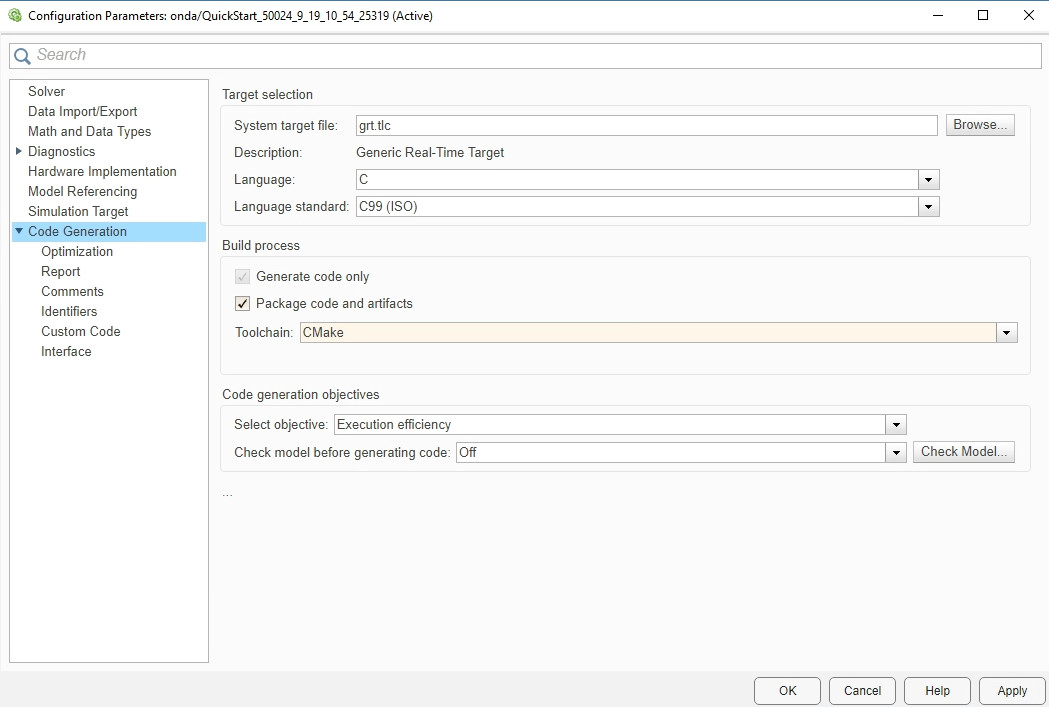
\includegraphics[width=0.8\textwidth]{fig/especifico_2/paso_a_paso_mtmt/configuration_output_file.png}
    \caption{Selección del tipo de archivo de construcción}
    \label{fig:pestana_config_output_file}
\end{figure}

\subsubsection{Generación de archivos de compilación}

Una vez configurados todos los parámetros mencionados anteriormente debemos de proceder con la construcción de los archivos, para esto se debe de ir a la barra de tareas a la opción denominada como generar código, la misma se puede observar en la Figura \ref{fig:pestana_c_code} bajo el nombre de Build.

\begin{figure}[h!]
    \centering
    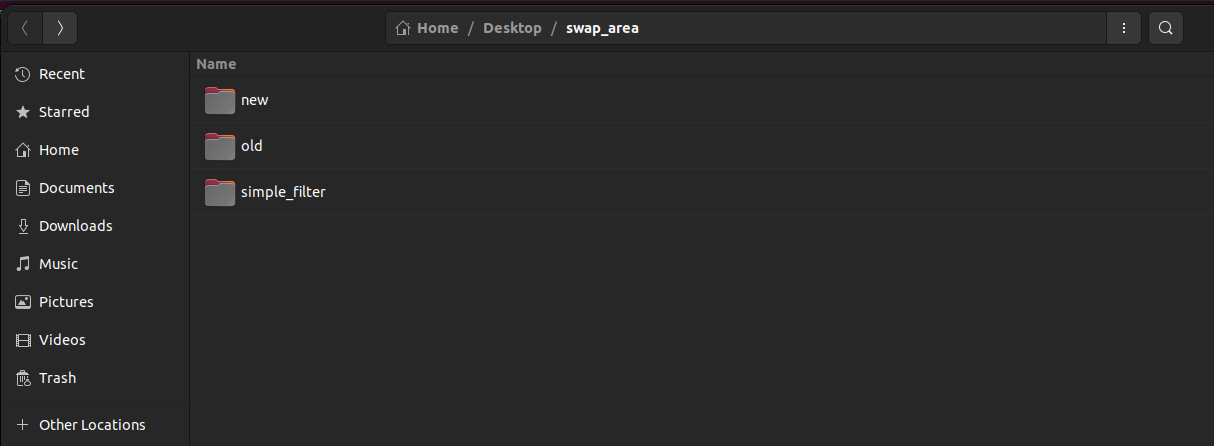
\includegraphics[width=0.8\textwidth]{fig/especifico_2/paso_a_paso_mtmt/root_folder.png}
    \caption{Archivo comprimido en el directorio swap\_area}
    \label{fig:pestana_swap_area}
\end{figure}

\begin{lstlisting}[language=bash, caption={Copiar archivos al contenedor, Linux}, label=lst:copy_to_container]
    sudo docker cp /direccion/del/archivo 
    <id_de_contenedor>:/direccion/del/contenedor
\end{lstlisting}

\begin{lstlisting}[language=bash, caption={Copiar archivos del contenedor, Linux}, label=lst:copy_from_container]
    sudo docker cp <id_de_contenedor>:/direccion/del/contenedor
    /direccion/del/archivo
\end{lstlisting}

Seguido de esto se debe de copiar el archivo comprimido generado en \ref{subsec:simulink_coder}, al contenedor con Ubuntu. Primeramente colocaremos el archivo comprimido en un directorio llamado swap\_area, tal y como se muestra en \ref{fig:pestana_swap_area}. Seguido de esto se debe de descomprimir el archivo. Una vez descomprimido el archivo, como se mencionó anteriormente, lo enviaremos al contenedor haciendo uso del comando \ref{lst:copy_to_container}.

\subsection{Compilación de los binarios}\label{subsec:compilacion_binario}

\begin{lstlisting}[language=bash, caption={Compilacion del programa, Linux}, label=lst:build_cmake_file]
    cmake -DCMAKE_C_COMPILER=arm-linux-gnueabihf-gcc 
    CMakeLists.txt -DMATLAB_ROOT=/home/test/simple_filter/R2024b/
\end{lstlisting}

\begin{figure}[h!]
    \centering
    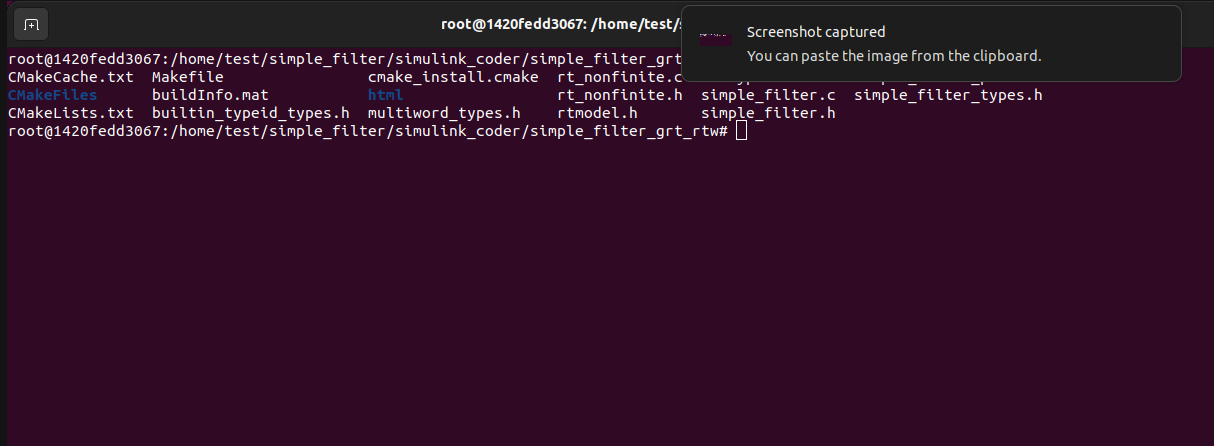
\includegraphics[width=0.8\textwidth]{fig/especifico_2/paso_a_paso_mtmt/cmake_file.png}
    \caption{Make File}
    \label{fig:make_file}
\end{figure}


\begin{figure}[h!]
    \centering
    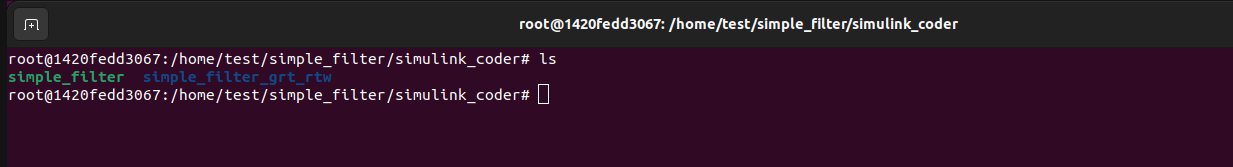
\includegraphics[width=0.8\textwidth]{fig/especifico_2/paso_a_paso_mtmt/binario_compilado.png}
    \caption{Binario llamado simple\_filter}
    \label{fig:binario_compilado}
\end{figure}

Para la compilación del archivo binario se deberá hace uso del comando \ref{lst:build_cmake_file} por el cual se construirá el Makefile, tal y como se muestra en la Figura \ref{fig:make_file}, una vez generado el Makefile se ejecutó el comando make el cual da como salida los binarios requeridos para la ejecución del programa. Los mismos se observan como se muestra en la Figura \ref{fig:binario_compilado}.

Una vez compilado el archivo binario, se puede continuar con el flujo que se presenta en el diagrama que se muestra en la Figura \ref{fig:diagrama_flujo_trabajo}, lo cual sería la implementación de los binarios en una imagen de yocto.


\section{Flujo de Trabajo EmbedSynthGNC}

Como se pudo observar anteriormente se realizó la compilación cruzada de un caso de estudio, el mismo ahora se debe de implementar en un sistema operativo a la medida mediante el flujo de trabajo de Yocto Project, como se mencionó en \ref{subsec:yocto}, Yocto Project es un marco de trabajo utilizado para el desarrollo de sistemas embebidos especializado en la construcción de distribuciones de Linux a la medida. 

\begin{figure}[h!]
    \centering
    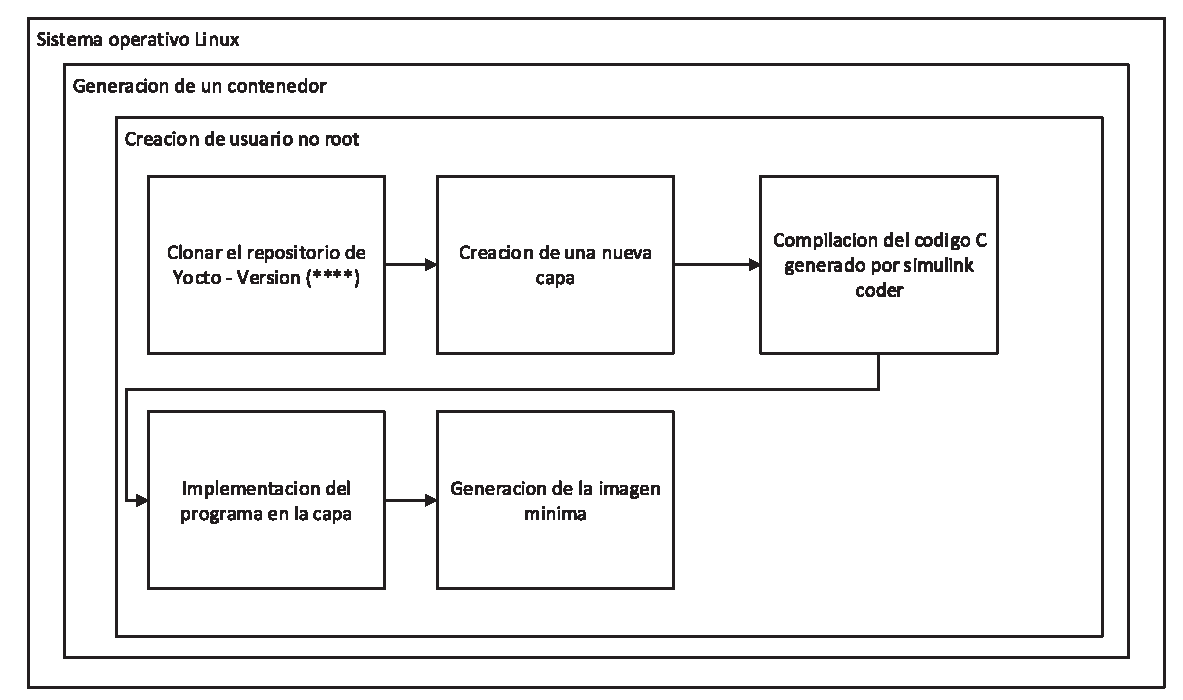
\includegraphics[width=0.8\textwidth]{fig/especifico_2/Flujo de trabajo de mi idea.pdf}
    \caption{Flujo de trabajo Yocto}
    \label{fig:flujo_yocto}
\end{figure}

En el desarrollo de esta sección se muestran los pasos que se siguieron para la generación de una imagen, la integración de una capa personalizada con el binario generado en \ref{subsec:compilacion_binario} y la implementación de la misma en la tarjeta de desarrollo seleccionada.

\subsection{Creación de una capa de yocto}

\begin{lstlisting}[language=bash, caption={"Print Working Directory",Linux}, label=lst:pwd]
    pwd
\end{lstlisting}

\begin{lstlisting}[language=bash, caption={Inicializar ambiente, Yocto}, label=lst:yocto_ambient_set]
    source oe-init-build-env
\end{lstlisting}

Para la generación de una capa de yocto primero debemos de estar seguros que nos encontramos en el directorio denominado POKY, esto lo podemos verificar por medio del uso del comando \ref{lst:pwd}, seguido de esto se debe de inicializar el entorno de desarrollo esto mediante el comando que se muestra en \ref{lst:yocto_ambient_set}, este se encarga de generar todos los archivos necesarios para poder hacer uso de las variables de entorno con las cuales opera el marco de trabajo de Yocto.

\begin{lstlisting}[language=bash, caption={Generar nueva capa, Yocto }, label=lst:yocto_new_layer]
    bitbake-layers create-layer <nombre-de-la-capa>
\end{lstlisting}

\begin{figure}[h!]
    \centering
    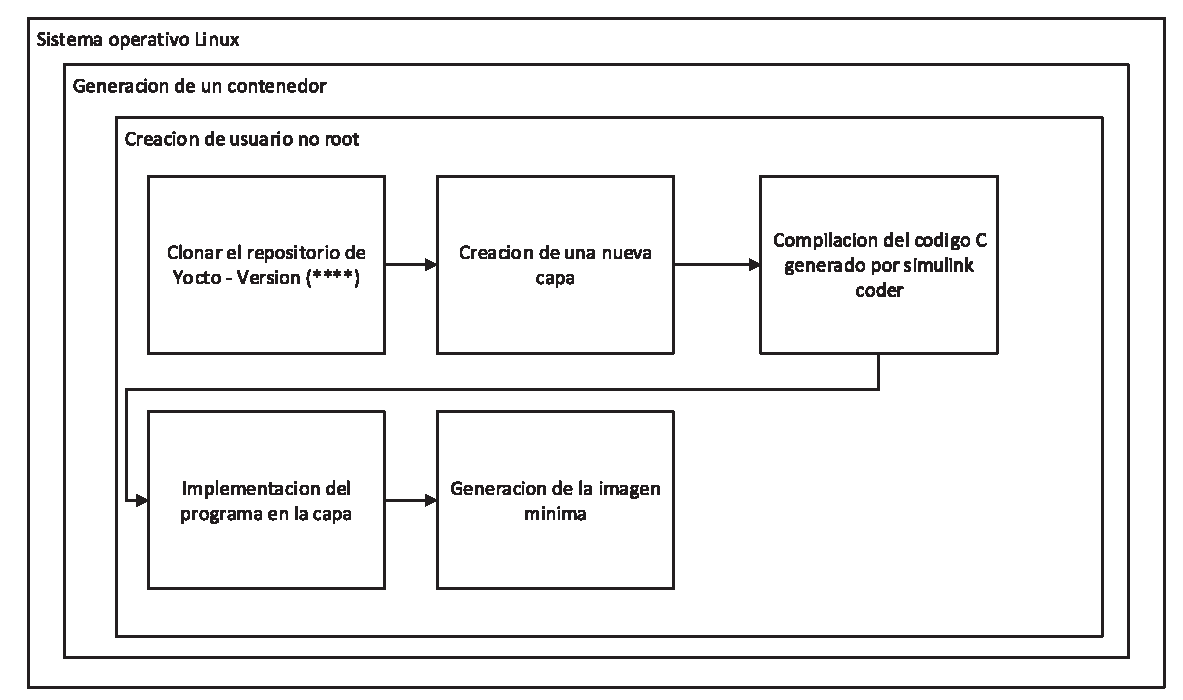
\includegraphics[width=0.8\textwidth]{fig/especifico_2/Flujo de trabajo de mi idea.pdf}
    \caption{Árbol de directorios de la capa}
    \label{fig:arbol_capa_custom_yocto}
\end{figure}

\begin{lstlisting}[language=bash, caption={Agregar nueva capa, Yocto }, label=lst:add_new_layer]
    bitbake-layers add-layer ../<nombre-de-la-capa>
\end{lstlisting}

Seguido de esto se debe de utilizar el comando que se muestra en \ref{lst:yocto_new_layer} el cual se encargara de generar el árbol de directorios que se puede observar en la Figura \ref{fig:arbol_capa_custom_yocto}. Una vez implementado este comando se debe de hacer uso del comando que se muestra en \ref{lst:add_new_layer} para poder agregar la capa al archivo denominado bblayers.conf el cual contiene todas las rutas de acceso a las capas requeridas para generar la imagen.

\subsection{Caso de estudio}

En esta sección se integrará el caso de estudio generado en \ref{subsec:compilacion_binario}, a un sistema operativo a la medida por medio del marco de trabajo de Yocto Project, primeramente se generara una capa personalizada, seguido de esto se generara el archivo de instalación con el cual la capa personalizada pasara a ser parte del sistema de archivos del sistema embebido, también se generara la imagen mínima la cual consiste en un sistema de arranque y el sistema de archivos y finalmente se implementaran estos en la tarjeta de desarrollo seleccionada en \ref{ch:especifico1}.

\subsection{Integración del programa generado a la capa de Yocto}

Para la implementación del binario generado en \ref{subsec:compilacion_binario}, se deben de generar algunos directorios, esto con el objetivo de mantener un entorno limpio y ordenado. Para contener todos los directorios que se deben de crear, se genera un directorio llamado "recipes-core" el cual dentro del mismo deberá de contener un directorio llamado "sistema\_control" el cual se encargara de contener el archivo de configuración de la capa llamado "sistema\_control.bb"; este archivo se genera mediante el comando que se observa en \ref{lst:yocto_new_layer}, además de generar este archivo se debe de crear un directorio llamado "files" que será el encargado de contener el archivo binario compilado en \ref{subsec:compilacion_binario}.

\subsubsection{sistema\_control.bb}

Como se mencionó anteriormente el archivo llamado sistema\_control.bb es el encargado de la configuración de la capa, el mismo contiene los comandos de instalación y la dirección en donde se encontraran los binarios en el sistema de archivos de la imagen del sistema embebido.

\begin{figure}[h!]
    \centering
    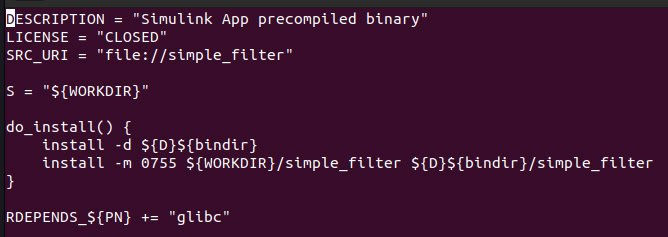
\includegraphics[width=0.8\textwidth]{fig/especifico_2/bbfilestructure.jpg}
    \caption{Estructura del archivo sistema\_control.bb}
    \label{fig:estructura_archivo_bb}
\end{figure}

La estructura que debe de contener ese archivo para instalar binarios en el sistema son las que se pueden observar en la Figura \ref{fig:estructura_archivo_bb}.

\subsection{Generación de la imagen mínima}\label{subsec:generacion_imagen_minima}

\begin{lstlisting}[language=bash, caption={Generar archivos de desarrollador, Yocto }, label=lst:yocto_developer_image]
    bitbake-layers add-layer ../<nombre-de-la-capa>
\end{lstlisting}

Antes de generar la imagen mínima se debe de tener en consideración ejecutar la línea de comando que se muestra en \ref{lst:yocto_developer_image}, esto con el fin de generar archivos de desarrollo en lugar de archivos de imagen en formato iso. Una vez generados estos cambios se debe de iniciar de nuevo el entorno por medio del comando \ref{lst:yocto_ambient_set}, seguido de esto se deberá de ejecutar el comando de "bitbake core-image-minimal" el cual se encarga de comenzar a generar la imagen mínima.

\subsection{Implementación de la imagen mínima en la tarjeta de desarrollo Zedboard}

Para la implementación de la imagen mínima desarrollada en \ref{subsec:generacion_imagen_minima} en la tarjeta de desarrollo, se deben de desarrollar los siguientes pasos en la máquina Host:

\begin{enumerate}
    \item Se debe de formatear la tarjeta SD de al menos 4 GB, las particiones de la misma se tienen que observar de la siguiente forma 
    \begin{itemize}
        \item raíz = 100 MB FAT 32
        \item sistema de archivos = 3.5 GB ext6(linux filesystem format)
        \end{itemize} 
\end{enumerate}

Seguido de esto se debe de ir a la ruta (ruta donde se encuentran los archivos de imagen de la zedboard), mientras que en la máquina host se debe de ir a la ruta seleccionada para almacenar los archivos temporalmente y se deben de copiar los archivos del contenedor a la máquina host mediante el comando que se muestra en \ref{lst:copy_from_container}, esto con el objetivo de poder enviar los archivos a la tarjeta SD más adelante.

\begin{lstlisting}[language=bash, caption={Copiar archivos root, Linux}, label=lst:copy_root]
    sudo cp boot.bin boot.scr 
    core-image-minimal-zedboard-zynq7.cpio.gz.u-boot
     u-boot.img uEnv.txt uImage zynq-zed.dtb /media/root
\end{lstlisting}

\begin{lstlisting}[language=bash, caption={Copiar sistema de archivos, Linux}, label=lst:copy_fs]
    sudo cp core-image-minimal-zedboard-zynq7.tar.gz /mnt/partition2
\end{lstlisting}

Para el sistema Root se deberán de copiar los archivos mediante el comando que se muestra en \ref{lst:copy_root}, por otro lado en la partición denominada FileSystem se debe de copiar el archvivo "core-image-minimal-zedboard-zynq7.tar.gz" mediante el uso del comando que se muestra en \ref{lst:copy_fs}.

\subsection{Conexión de la tarjeta de desarrollo con el computador host}

Como protocolo de comunicación se establece de primera mano UART, el cual como se mencionó en \ref{sec:protocolos_de_comunicacion} consiste en un protocolo de comunicación serie que permite la transmisión y recepción de datos de manera asíncrona entre dos dispositivos y en el caso de la tarjeta de desarrollo se conecta según se muestra en el diagrama de la Figura \ref{fig:puertos_zedboard}, mediante el uso del puerto marcado como "S" en el diagrama. Para poder leer la consola se hace uso de Minicom el cual se encarga de la emulación de terminal en Linux que permite la comunicación serie con dispositivos a través de puertos seriales.

\begin{figure}[h!]
    \centering
    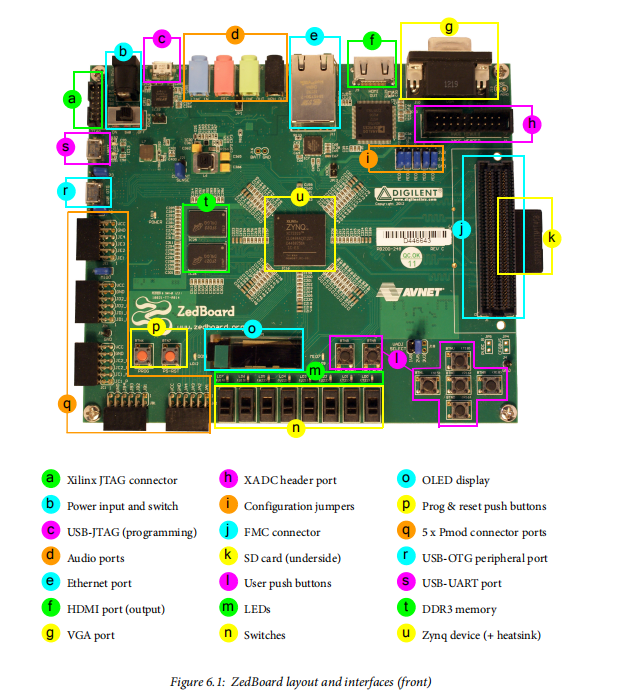
\includegraphics[width=0.8\textwidth]{fig/especifico_2/154140ZedBoard.png}
    \caption{Puertos tarjeta de desarrollo Zedboard}
    \label{fig:puertos_zedboard}
\end{figure}


Una vez que se estableció la conexión por medio de SSH el cual como se menciona en \ref{sec:protocolos_de_comunicacion}, consiste en protocolo de comunicación en red que permite el acceso remoto seguro a sistemas, proporcionando autenticación y encriptación de datos, ya que es mejor que UART para comunicaciones remotas porque proporciona autenticación y encriptación, garantizando la seguridad de los datos transmitidos, mientras que UART es un protocolo simple y sin mecanismos de seguridad, adecuado solo para comunicaciones locales y de corto alcance. 

El diagrama de este protocolo de comunicación se puede observar en \ref{fig:puertos_zedboard}, el cual se logra mediante la conexión al puerto denominado en el diagrama como e.


\subsection{Ejecución del caso de estudio y resultados}

Una vez implementada la imagen de Yocto en la tarjeta de desarrollo se puede ejecutar el caso de estudio. Para esto será necesario dirigirnos al directorio en el cual se instaló el archivo binario, el mismo se encuentra en la ruta usr-bin-simple\_filter. Una vez encontrado el archivo basta con ejecutarlo mediante el uso del nombre del mismo simple\_filter. Cuando el archivo se ejecuta genera dos archivos de salida llamados Raw\_signal.mat y Filtered\_signal.mat, mediante el uso del programa en Python desarrollado se pueden leer los archivos generados y crear gráficos a partir de los mismos. Los resultados se deben de transmitir al computador por medio del comando \ref{lst:copy_ssh}.

\begin{lstlisting}[language=bash, caption={Copiar archivo por protocolo SSH, Linux}, label=lst:copy_ssh]
    scp user@ip:/ruta/del/archivo/zedboard .
\end{lstlisting}

\begin{figure}[htbp]
    \centering
    \begin{subfigure}[b]{0.45\textwidth}
        \centering
        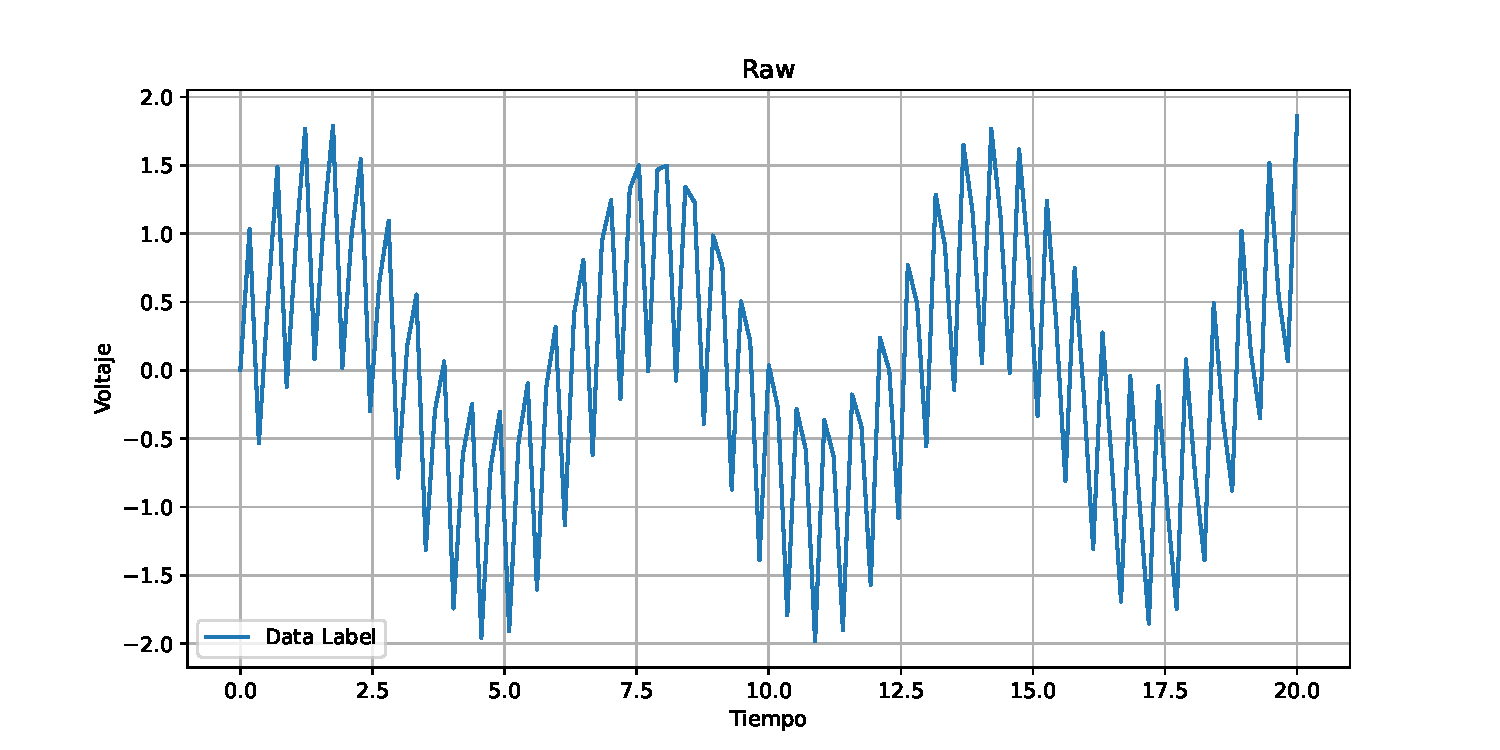
\includegraphics[width=\textwidth]{fig/especifico_2/raw.pdf}
        \caption{Ondas Moduladas}
        \label{fig:onda_modulada_zedboard}
    \end{subfigure}
    \hfill
    \begin{subfigure}[b]{0.45\textwidth}
        \centering
        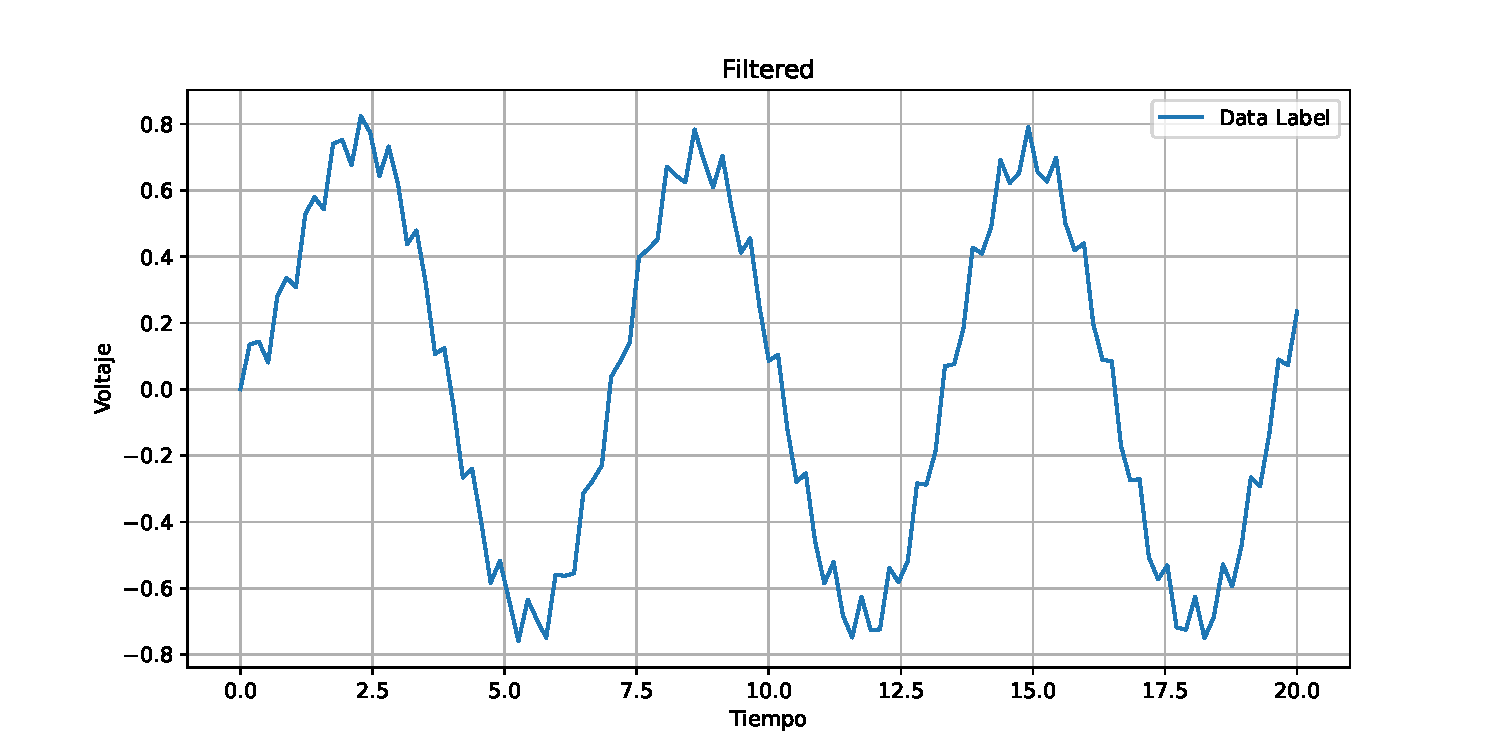
\includegraphics[width=\textwidth]{fig/especifico_2/Filtered.pdf}
        \caption{Onda resultante luego de la función de transferencia}
        \label{fig:onda_filtrada_zedboard}
    \end{subfigure}
    \caption{Salida resultante de la imagen generada mediante el flujo de trabajo}
    \label{fig:salida_resultante_diagrama_graficos_zedboard}
\end{figure}

\subsection{Comparación de resultados}



\section{Reflexión final}